% TODO: Dodělat
\documentclass{szzclass}
\usepackage{hyperref}
\usepackage{dependencies/szz-code}

% \subject{TJV}
% \code{BI-WSI-SI-29}
% \topic{Aplikační server a JNDI služba: popis aplikačního serveru, webový kontejner, EJB kontejner, využití JNDI ke konfiguraci datových zdrojů.}

\begin{document}

\section{Aplikační server}
\begin{itemize}
\item Serverovou aplikaci zastřešující všechny knihovny, které dle specifikací Java EE platformy zajišťují požadovanou funkcionalitu, označujeme pojmem aplikační server. 
\item Tyto knihovny implementují veškerá API obsažená v Java EE. 
\item Kromě toho poskytuje aplikační server další klasické služby jako např. 
  \begin{itemize}
    \item administrátorskou konzoli, 
    \item logování atp. 
  \end{itemize}
\item Ze známých implementací Java EE platformy můžeme zmínit např. JBoss od firmy Red Hat či JRun od firmy Adobe Systems. Referenční implementace Oracle je šířena pod hlavičkou projektu GlassFish.
\item Zajišťuje:
  \begin{itemize}
    \item Vývoj webových aplikací - Java Servlets, Java Server Pages (JSP), JavaServer Faces (JSF)
    \item Contexts and Dependency Injection - vkládání závislostí
    \item Přístup k relačním databázím - Java Persistence API (ORM)
    \item Vývoj sdílené business logiky - Enterprise Java Beans (EJB)
    \item Přístup k legacy systémům - Java Connector Architecture (JCA)
    \item Přístup ke zprávovému middleware - Java Messaging Services (JMS)
    \item Komponenty zajišťující integraci webových aplikací a portálů - Portlety
    \item Podpora technologií Webových služeb- SOA, REST
  \end{itemize}
\end{itemize}

\begin{figure}[ht!]
\centering
\begin{minipage}{.5\textwidth}
  \centering
  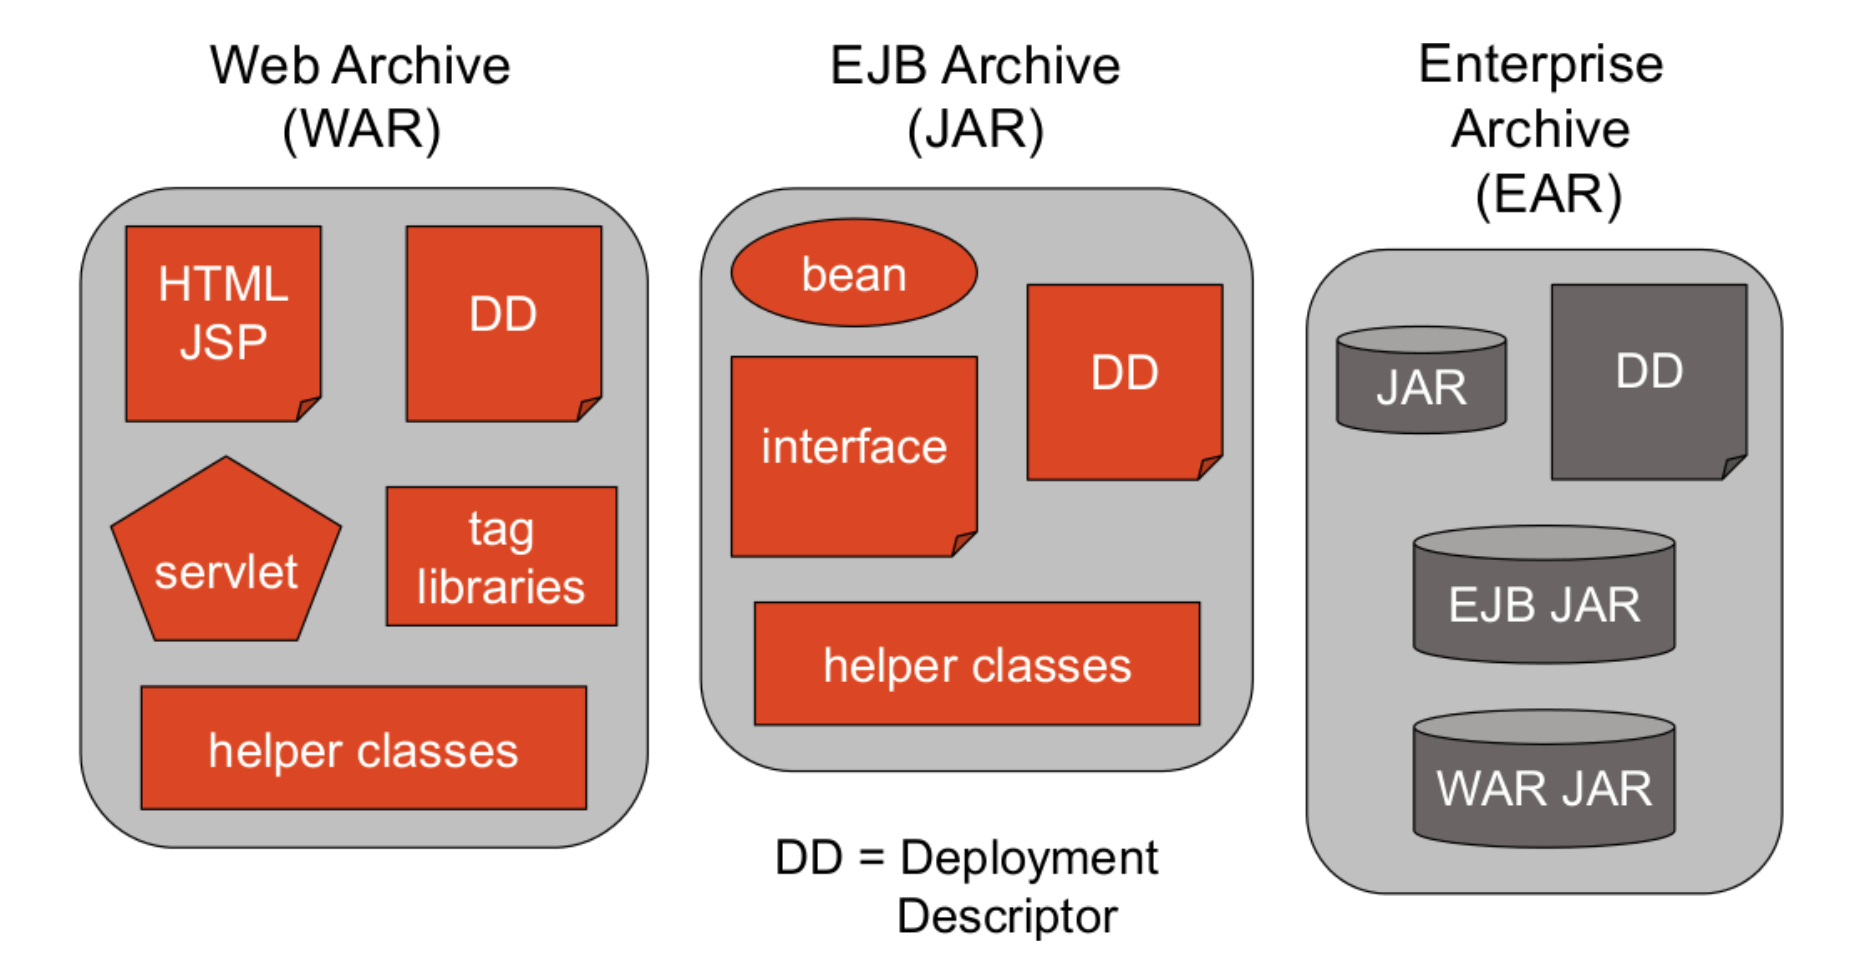
\includegraphics[width=.75\linewidth]{topics/bi-wsi-si-29/images/image1}
\end{minipage}%
\begin{minipage}{.5\textwidth}
  \centering
  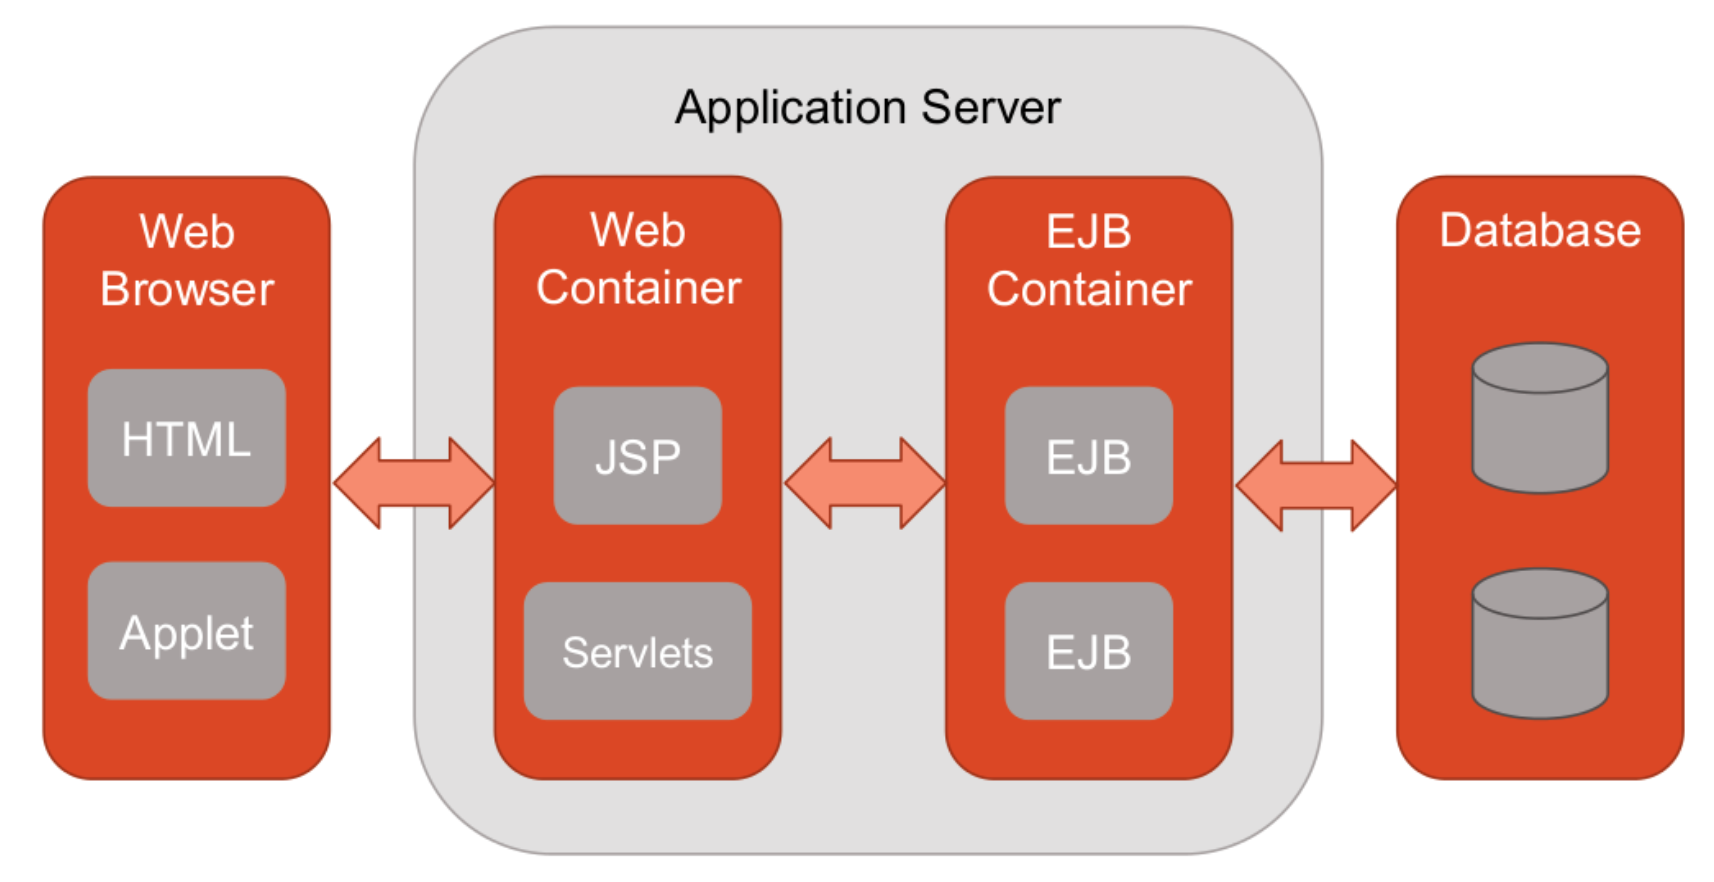
\includegraphics[width=.75\linewidth]{topics/bi-wsi-si-29/images/image2}
\end{minipage}
\end{figure}

Aplikační server obsahuje dva kontejnery - webový a EJB. Ty obsahují komponenty, instantizují je a řídí jejich životní cyklus. Komponenty nemohou žít bez kontejneru.

Výsledkem je .ear balíček, který je vytvořen třeba vývojovým prostředím za pomocí Mavenu, Antu nebo novějšího Gradlu. Všechny tři zmíněné nástroje jsou tzv. build systémy. Další ze známějších je Make (známe z BI-PA2), ale ten se tady nepoužívá.

EJB komponenty
\begin{itemize}
\item Odpovídá business vrstvě z otázky \href{https://docs.google.com/document/d/1OU75LDsImR4cEsQoyfGNyibG5ECJhGRKCfJqrUlpl1Q/edit?usp=sharing}{architektura aplikací}
\item Více o EJB v otázce \href{https://docs.google.com/document/d/1_yV6LyQ3dHi9VSOQhmPtGe9QXRESZDfxDK_NA9gJ1dY/edit?usp=sharing}{EJB}
\item Balíček jar
\end{itemize}

Webový kontejner (podobně jako EJB kontejner - viz \href{https://docs.google.com/document/d/1_yV6LyQ3dHi9VSOQhmPtGe9QXRESZDfxDK_NA9gJ1dY/edit?usp=sharing}{EJB} otázka)
\begin{itemize}
\item Mapuje URL adresy na servlety
\item Zajišťuje bezpečnost - může uživatel přistoupit k danému kontejneru?
\item Řídí životní cyklus servletů - vytváření, mazání
\item Pracuje s dotazy a odpověďmi serveru
\item Spravuje pool servletů
\end{itemize}

Webové komponenty
\begin{itemize}
\item odpovídá definici webové vrstvy z otázky \href{https://docs.google.com/document/d/1OU75LDsImR4cEsQoyfGNyibG5ECJhGRKCfJqrUlpl1Q/edit?usp=sharing}{architektura aplikací}
\item Balíček .war
\end{itemize}

\section{JNDI}
Java Naming and Directory Interface

Aplikační server zajišťuje službu JNDI. Ta na základě klíčového slova (unikátního názvu zdroje) zajistí vyhledání a předání existující konfigurace žádající aplikaci. Využívá se třeba pro získání instance EJB nebo DataSource (pro připojení k databázi).

Aplikační server dále zajišťuje připojení ke zdroji a obnovení komunikace, pokud se něco podělá. Pro získání instancí slouží třída \mintinline{java}{InitialContext}, kterou si můžeme kdykoliv vytvořit.

Pomocí metody \mintinline{java}{InitialContext#lookup(Name)} lze získat instanci objektu. Pokud pracujeme s databází, tak je potřeba v nastavení aplikačního serveru nastavit příslušný JDBC Resource a dát mu JNDI jméno (String) - viz otázka \href{https://docs.google.com/document/d/1Wfd-xg3CgY6YCLi15wh3ngDN0sPNNcg3bplWePlXTwM/edit}{JDBC}.

Jméno EJB je generováno automaticky ze jména třídy a umístění.

\begin{minted}[breaklines]{java}
  InitialContext ic = new InitialContext();
DataSource source = (DataSource) ic.lookup("jdbc/my_resouce_name");
MyBean bean = (MyBean) in.lookup("java:com/env/MyBean");
\end{minted}

\section{Zdroje}
Celý převzato z \url{https://docs.google.com/document/d/1evSul3rqDN7tW3vGMGhhVU4zNZFyCG-UumF0IdALn7g/edit#}
\begin{itemize}
\item BI-TJV 4. Přednáška \url{https://docs.google.com/presentation/d/12jr7jnWbx_S4sIwLd0v9HmUyX1uuAP3-z6HOdIDp7WA/edit}
\item BI-TJV 6. Přednáška \url{https://docs.google.com/presentation/d/1BdOU84Edw5YG3n7MVhsPQMTBGMV6_siDf6-sABXUTKk/edit}
\item JNDI - Wikipedia \url{https://en.wikipedia.org/wiki/Java_Naming_and_Directory_Interface}
\end{itemize}
\end{document}
